\documentclass[12pt]{article}

\usepackage[a4paper,margin=1in]{geometry}
\usepackage{amsmath,amssymb}
\usepackage{enumitem}
\usepackage{tikz}
\usepackage{circuitikz}
\usepackage{physics}
\usepackage{siunitx}
\usetikzlibrary{arrows.meta,angles,quotes,calc}

\setlist[enumerate]{itemsep=2em}


\begin{document}

\begin{center}
\Large \textbf{JEE ADVANCED – ABSOLUTE FINAL TIER}\\
\large Wave Optics \quad • \quad Modern Physics \quad • \quad Electronic Devices
\end{center}

\vspace{0.5cm}

\begin{enumerate}

%========================================================
\item In a Young’s double slit experiment (slit separation $d$, screen distance $D$), 
electrons accelerated through potential $V$ produce an interference pattern governed by their de Broglie wavelength. 

If the accelerating potential is increased slightly by $\Delta V$, the observed fringe width decreases by $0.5\%$. 
Neglect relativistic effects and assume small fractional changes.

Determine $\dfrac{\Delta V}{V}$.
\begin{center}
\begin{tikzpicture}[scale=1]

% Slits
\draw (-2,1.2)--(-2,0.8);
\draw (-2,-0.8)--(-2,-1.2);

% Slit center-to-center separation (d)
\draw[<->] (-2.4,1)--(-2.4,-1);
\node[left] at (-2.4,0) {$d$};

% Screen
\draw (3,-2)--(3,2);

% Screen distance arrow (D)
\draw[<->] (-2,-1.8)--(3,-1.8);
\node at (0.5,-2.2) {$D$};


% Electron paths
\draw[->] (-2,1)--(3,1.3);
\draw[->] (-2,-1)--(3,-0.4);

\node at (-2.8,0) {Double Slits};
\node[right] at (3,0) {Screen};

\end{tikzpicture}
\end{center}

A) $1\%$ \quad
B) $0.5\%$ \quad
C) $0.25\%$ \quad
D) $2\%$ \quad
E) $0.125\%$

%========================================================
\item In YDSE, each slit has finite width $a$ and separation $d$. 
Exactly five interference maxima (including the central maximum) lie inside the central diffraction envelope. 

Using the conditions for interference maxima and first diffraction minimum, determine $a/d$.

\begin{center}
\begin{tikzpicture}[scale=1]

% Upper slit
\draw (-2,0.7) rectangle (-1.8,1.7);

% Lower slit
\draw (-2,-1.7) rectangle (-1.8,-0.7);

% Mark slit centers
\coordinate (C1) at (-1.9,1.2);
\coordinate (C2) at (-1.9,-1.2);

% Width label (a)
\draw[<->] (-2,1.9)--(-1.8,1.9);
\node[above] at (-1.9,1.9) {$a$};

% Center-to-center separation (d)
\draw[<->] (-2.5,1.2)--(-2.5,-1.2);
\node[left] at (-2.5,0) {$d$};

% Mark centers visually
\fill (C1) circle (1.2pt);
\fill (C2) circle (1.2pt);

% Screen
\draw (3,-2)--(3,2);
\node at (3.6,0) {Screen};

\end{tikzpicture}
\end{center}

A) $1/5$ \quad
B) $1/4$ \quad
C) $1/3$ \quad
D) $2/5$ \quad
E) $1/6$

%========================================================
\item Unpolarized light is incident on a dielectric surface at an angle 
$\theta = \theta_B + \epsilon$, where $\theta_B$ is Brewster angle and $\epsilon$ is small. 

Using small-angle reasoning near Brewster angle, determine the lowest power of $\epsilon$ governing reflected intensity of the parallel component.

%================ Q3 Diagram =================
\begin{center}
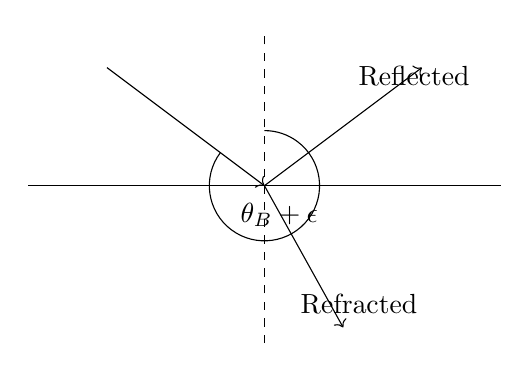
\begin{tikzpicture}[scale=1]

% Interface
\draw (-3,0)--(3,0);

% Normal
\draw[dashed] (0,-2)--(0,2);

% Incident ray
\draw[->] (-2,1.5)--(0,0);

% Reflected ray
\draw[->] (0,0)--(2,1.5);

% Refracted ray
\draw[->] (0,0)--(1,-1.8);

\coordinate (I) at (-2,1.5);
\coordinate (O) at (0,0);
\coordinate (N) at (0,1);

\pic [draw, "$\theta_B+\epsilon$", angle radius=0.7cm]
{angle = I--O--N};

\node at (1.9,1.4) {Reflected};
\node at (1.2,-1.5) {Refracted};

\end{tikzpicture}
\end{center}

A) $0$ \quad
B) $1$ \quad
C) $2$ \quad
D) $3$ \quad
E) $4$

%========================================================
\item A single slit of width $a$ produces a diffraction pattern on a distant screen. 
Exactly half of the slit width is blocked uniformly from one side. 

Assuming uniform illumination and coherent superposition, determine the fraction of original central maximum intensity that remains.

%================ Q4 Diagram =================
\begin{center}
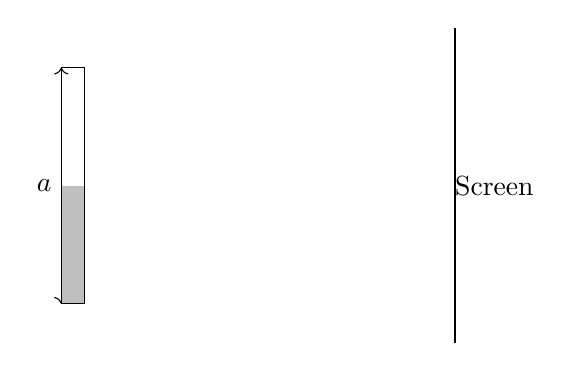
\begin{tikzpicture}[scale=1]
\draw (-2,-1.5) rectangle (-1.7,1.5);
\draw[<->] (-2,-1.5)--(-2,1.5);
\node[left] at (-2,0) {$a$};
\fill[gray!50] (-1.99,-1.49) rectangle (-1.71,0);

\draw (3,-2)--(3,2);
\node at (3.5,0) {Screen};
\end{tikzpicture}
\end{center}

A) $1/4$ \quad
B) $1/2$ \quad
C) $3/4$ \quad
D) $1$ \quad
E) $0$

%========================================================
\item A photocell is connected in series with resistor $R$ and battery $V_0$ opposing emission. 
Light frequency is slightly above threshold and intensity remains constant.

If frequency increases slightly while intensity is unchanged, determine which measurable quantity changes first.

%================ Q5 Diagram =================
\begin{circuitikz}
\draw
(0,0) -- (0,1)
(0,1) to[short] (0,2)
(0,2) -- (0,3)
(0,3) to[R,l=$R$] (3,3)
(3,3) to[battery,l_=$V$] (3,0)
(3,0) -- (0,0);

% Draw simple photocell plates manually
\draw (-0.4,1.2) -- (0.4,1.2);
\draw (-0.4,1.8) -- (0.4,1.8);
\node[left] at (-0.4,1.5) {Photocell};
\end{circuitikz}

A) Saturation current \quad
B) Stopping potential \quad
C) Both \quad
D) Neither \quad
E) Depends on $R$

%========================================================
\item In a photoelectric setup operating at saturation current, 
light intensity is doubled while frequency remains fixed above threshold. 

Determine change in electrical power delivered to the external circuit.

\begin{circuitikz}
\draw 
(0,0) to[photodiode,l=Photocell] (0,3)
      to[R,l=$R$] (3,3)
      to[battery,l_=$V$] (3,0)
      -- (0,0);
\end{circuitikz}

A) Doubles \quad
B) Same \quad
C) Halves \quad
D) Quadruples \quad
E) Depends on stopping potential

%========================================================
\item A radioactive sample has decay constant $\lambda$. 
Initial activity is $16A_c$, where $A_c$ is minimum detectable activity of a detector. 

Determine the fraction of total disintegrations that occur after the detector stops recording.

A) $1/16$ \quad
B) $15/16$ \quad
C) $1/4$ \quad
D) $3/4$ \quad
E) $1/2$

%========================================================
\item In hydrogen atom, the electron transitions from $n=4$ to $n=1$. 
Given that kinetic energy in $n^{\text{th}}$ orbit equals half the magnitude of total energy, determine ratio:

\[
\frac{E_{\text{photon}}}{K_{n=1}}
\]

A) $3$ \quad
B) $4$ \quad
C) $5$ \quad
D) $6$ \quad
E) $7$

%========================================================
\item An electron accelerated through potential $V$ enters a uniform magnetic field $B$ perpendicular to its velocity and moves in a circular path. 

If its de Broglie wavelength equals the radius of the circular orbit, determine scaling relation of $V$ with $B$.

%================ Q9 Diagram =================
\begin{center}
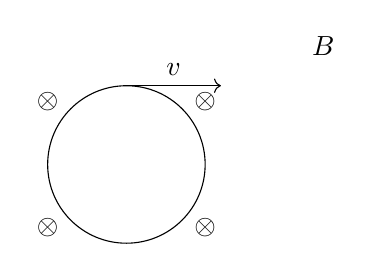
\begin{tikzpicture}[scale=1]

% Circle path
\draw (2,0) circle (1);

% Tangential velocity at entry point
\draw[->] (2,1)--(3.2,1) node[midway,above] {$v$};

% Magnetic field symbols
\node at (4.5,1.5) {$B$};
\foreach \x/\y in {1/0.8,3/0.8,1/-0.8,3/-0.8}
    \node at (\x,\y) {$\otimes$};

\end{tikzpicture}
\end{center}

A) $V \propto B$ \quad
B) $V \propto B^2$ \quad
C) $V \propto 1/B$ \quad
D) Independent of $B$ \quad
E) $V \propto 1/B^2$

%========================================================
\item A forward biased diode obeys 
\[
I = I_0\left(e^{\frac{eV}{kT}} - 1\right)
\]
A small AC voltage $v$ is superimposed on a DC bias $V$, where $v \ll V$. 

Using first-order expansion, determine amplitude of resulting AC current component.

A) $\dfrac{eI}{kT}v$ \quad
B) $\dfrac{kT}{eI}v$ \quad
C) $Iv$ \quad
D) $0$ \quad
E) $\dfrac{I_0 eV}{kT}v$

%========================================================
\item A diode in series with resistor $R$ is connected to a fixed battery $V_0$. 
Assuming exponential diode behavior and steady state, determine condition for maximum power dissipation in the resistor.
%================ Q11 Diagram =================
\begin{center}
\begin{circuitikz}
\draw (0,0) 
      to[battery,l=$V_0$] (0,4)
      to[R,l=$R$] (4,4)
      to[D, invert] (4,0) node[midway, right=4pt]{$D$}
      -- (0,0);
\end{circuitikz}
\end{center}

A) $R = r_d$ \quad
B) $R \to 0$ \quad
C) $R \to \infty$ \quad
D) $V_D = V_0/2$ \quad
E) No maximum exists

%========================================================
\item In a common emitter configuration with resistive load, 
base current increases slightly while the transistor remains in active region.

Assuming transistor current gain $\beta$ remains constant, determine instantaneous change in collector current.

%================ Q12 Diagram =================
\begin{center}
\begin{circuitikz}
\draw 
(0,0) node[npn,anchor=E](Q){}
(Q.B) node[left]{$B$}
(Q.E) node[below]{$E$}
(Q.E) -- ++(0,-1) node[ground]{}
(Q.C) -- ++(0,1) to[R,l=$R_C$] ++(0,2) node[above]{$V_{CC}$};
\end{circuitikz}
\end{center}



A) Increases \quad
B) Decreases \quad
C) No change \quad
D) Oscillates \quad
E) Depends on $\beta$

%========================================================
\item A half-wave rectifier with capacitor filter has ripple factor approximately
\[
r \propto \frac{1}{fRC}
\]

If $f \to 2f$, $R \to R/2$, and $C \to 2C$, determine new ripple relative to original.

%================ Q13 Diagram =================
\begin{center}
\begin{circuitikz}
\draw (0,0) to[sV,l=$AC$] (0,3)
      to[D] (3,3)
      to[R,l=$R$] (3,0)
      -- (0,0);
\draw (3,3) to[C,l=$C$] (3,0);
\end{circuitikz}
\end{center}

A) Same \quad
B) Half \quad
C) Double \quad
D) One-fourth \quad
E) Four times

%========================================================
\item In a diode-based AND gate, one input is fixed HIGH. 
The second input oscillates symmetrically about threshold voltage $V_T$.

Assuming ideal switching behavior, determine average logical output over one full oscillation cycle.

%================ Q14 Diagram =================
\begin{center}
\begin{circuitikz}
\draw 
(0,2) node[left]{$A$} to[D] (2,2)
(0,0) node[left]{$B$} to[D] (2,0)
(2,2) -- (2,0)
(2,2) -- ++(1.3,0) node[right]{Output}
(2,0) to[R,l=$R$] (2,-2) node[ground]{};
\end{circuitikz}
\end{center}

A) Always HIGH \quad
B) Always LOW \quad
C) 50\% HIGH \quad
D) Depends on amplitude \quad
E) Depends on frequency

%========================================================
\item Electrons accelerated through potential $V$ strike a metal target producing X-rays whose maximum frequency depends on $V$.

That light is used in a Young’s double slit experiment. If applied voltage increases slightly, determine direction of fringe shift on screen.

\begin{center}
\begin{tikzpicture}[scale=1]

% LED source
\node[left] at (-2.2,0) {X-ray Source};

% Slits
\draw (-1,0.7)--(-1,1.2);
\draw (-1,-1.2)--(-1,-0.7);

% Screen
\draw (3,-2)--(3,2);

% Rays
% Incident light
\draw[->] (-3,0)--(-1,0);

% Diffraction after slits
\draw[->] (-1,1)--(3,1.3);
\draw[->] (-1,-1)--(3,-0.4);
\end{tikzpicture}
\end{center}

A) Toward center \quad
B) Away from center \quad
C) No shift \quad
D) Oscillatory shift \quad
E) Depends on slit width

%========================================================

\end{enumerate}

\end{document}